
\chapter{Fundamental equations and processes}
\label{ch:fundamental-eqs-processes}

\lastupdated{2024-12-06}{\chapterTwoEqsProc}



The atmosphere and the ocean are both vast and dynamic systems that behave as fluids under the influence of a rotating planet. Although their physical properties differ—air being compressible and water being nearly incompressible—their motions can be described using the principles of fluid dynamics. These principles form the basis for understanding and predicting a wide range of phenomena, from local weather patterns to global climate dynamics.

In this chapter, we explore the fundamental equations that govern the behavior of these fluid systems. Starting from the basic conservation laws of momentum, mass, and energy, we show the governing equations for atmospheric and oceanic motion. Due to the complexity of these systems, certain approximations are often applied to make these equations tractable. These approximations include the hydrostatic approximation, the shallowness approximation, and the neglect of specific higher-order terms. Such simplifications allow us to focus on the dominant processes and forces shaping the dynamics of the atmosphere and the ocean.

We will discuss the mathematical framework and coordinate systems used to describe these systems, followed by the equations of motion and key approximations. Later sections will delve into the physical processes such as radiation, moisture, and hydrology that interact with the dynamics of the atmosphere and ocean.

\section{Background}\label{sec:intro-fund-eqs-processes}

\subsection{The Earth spherical coordinates system}
\label{subsec:spherical-coordinate-systems}
The most commonly used coordinate system for the analysis of the
atmosphere and the oceans is a spherical coordinate system attached to
the rotating Earth (\fig{\ref{fig:3d-coordinate-sys}}). The spherical coordinates are
slightly different from the usual mathematical ones as the latitude $\phi$ is
measured from the equator and therefore it can take negative values.
The longitude $\lambda$ is running west to east.

The longitude is also known as the \textbf{zonal} direction whereas the
latitude is also known as the \textbf{meridional} direction.
Winds are identified by the direction they are coming from, so a \emph{westerly} wind
is coming \emph{from} the West and an \emph{easterly} wind is coming \emph {from} the
East.

Hereafter we will denote with $\vec{\Omega} = \Omega \unitv{k}$ Earth's angular velocity vector, with $\Omega \simeq \qty{7.29e-5}{\radian \per \second}$.
Since this reference frame is rotating, it is necessary to add force terms in the dynamical equations (see Coriolis terms in~\eq{\ref{eq:momentum-eq-atm}}).
\begin{figure}
	\centering
	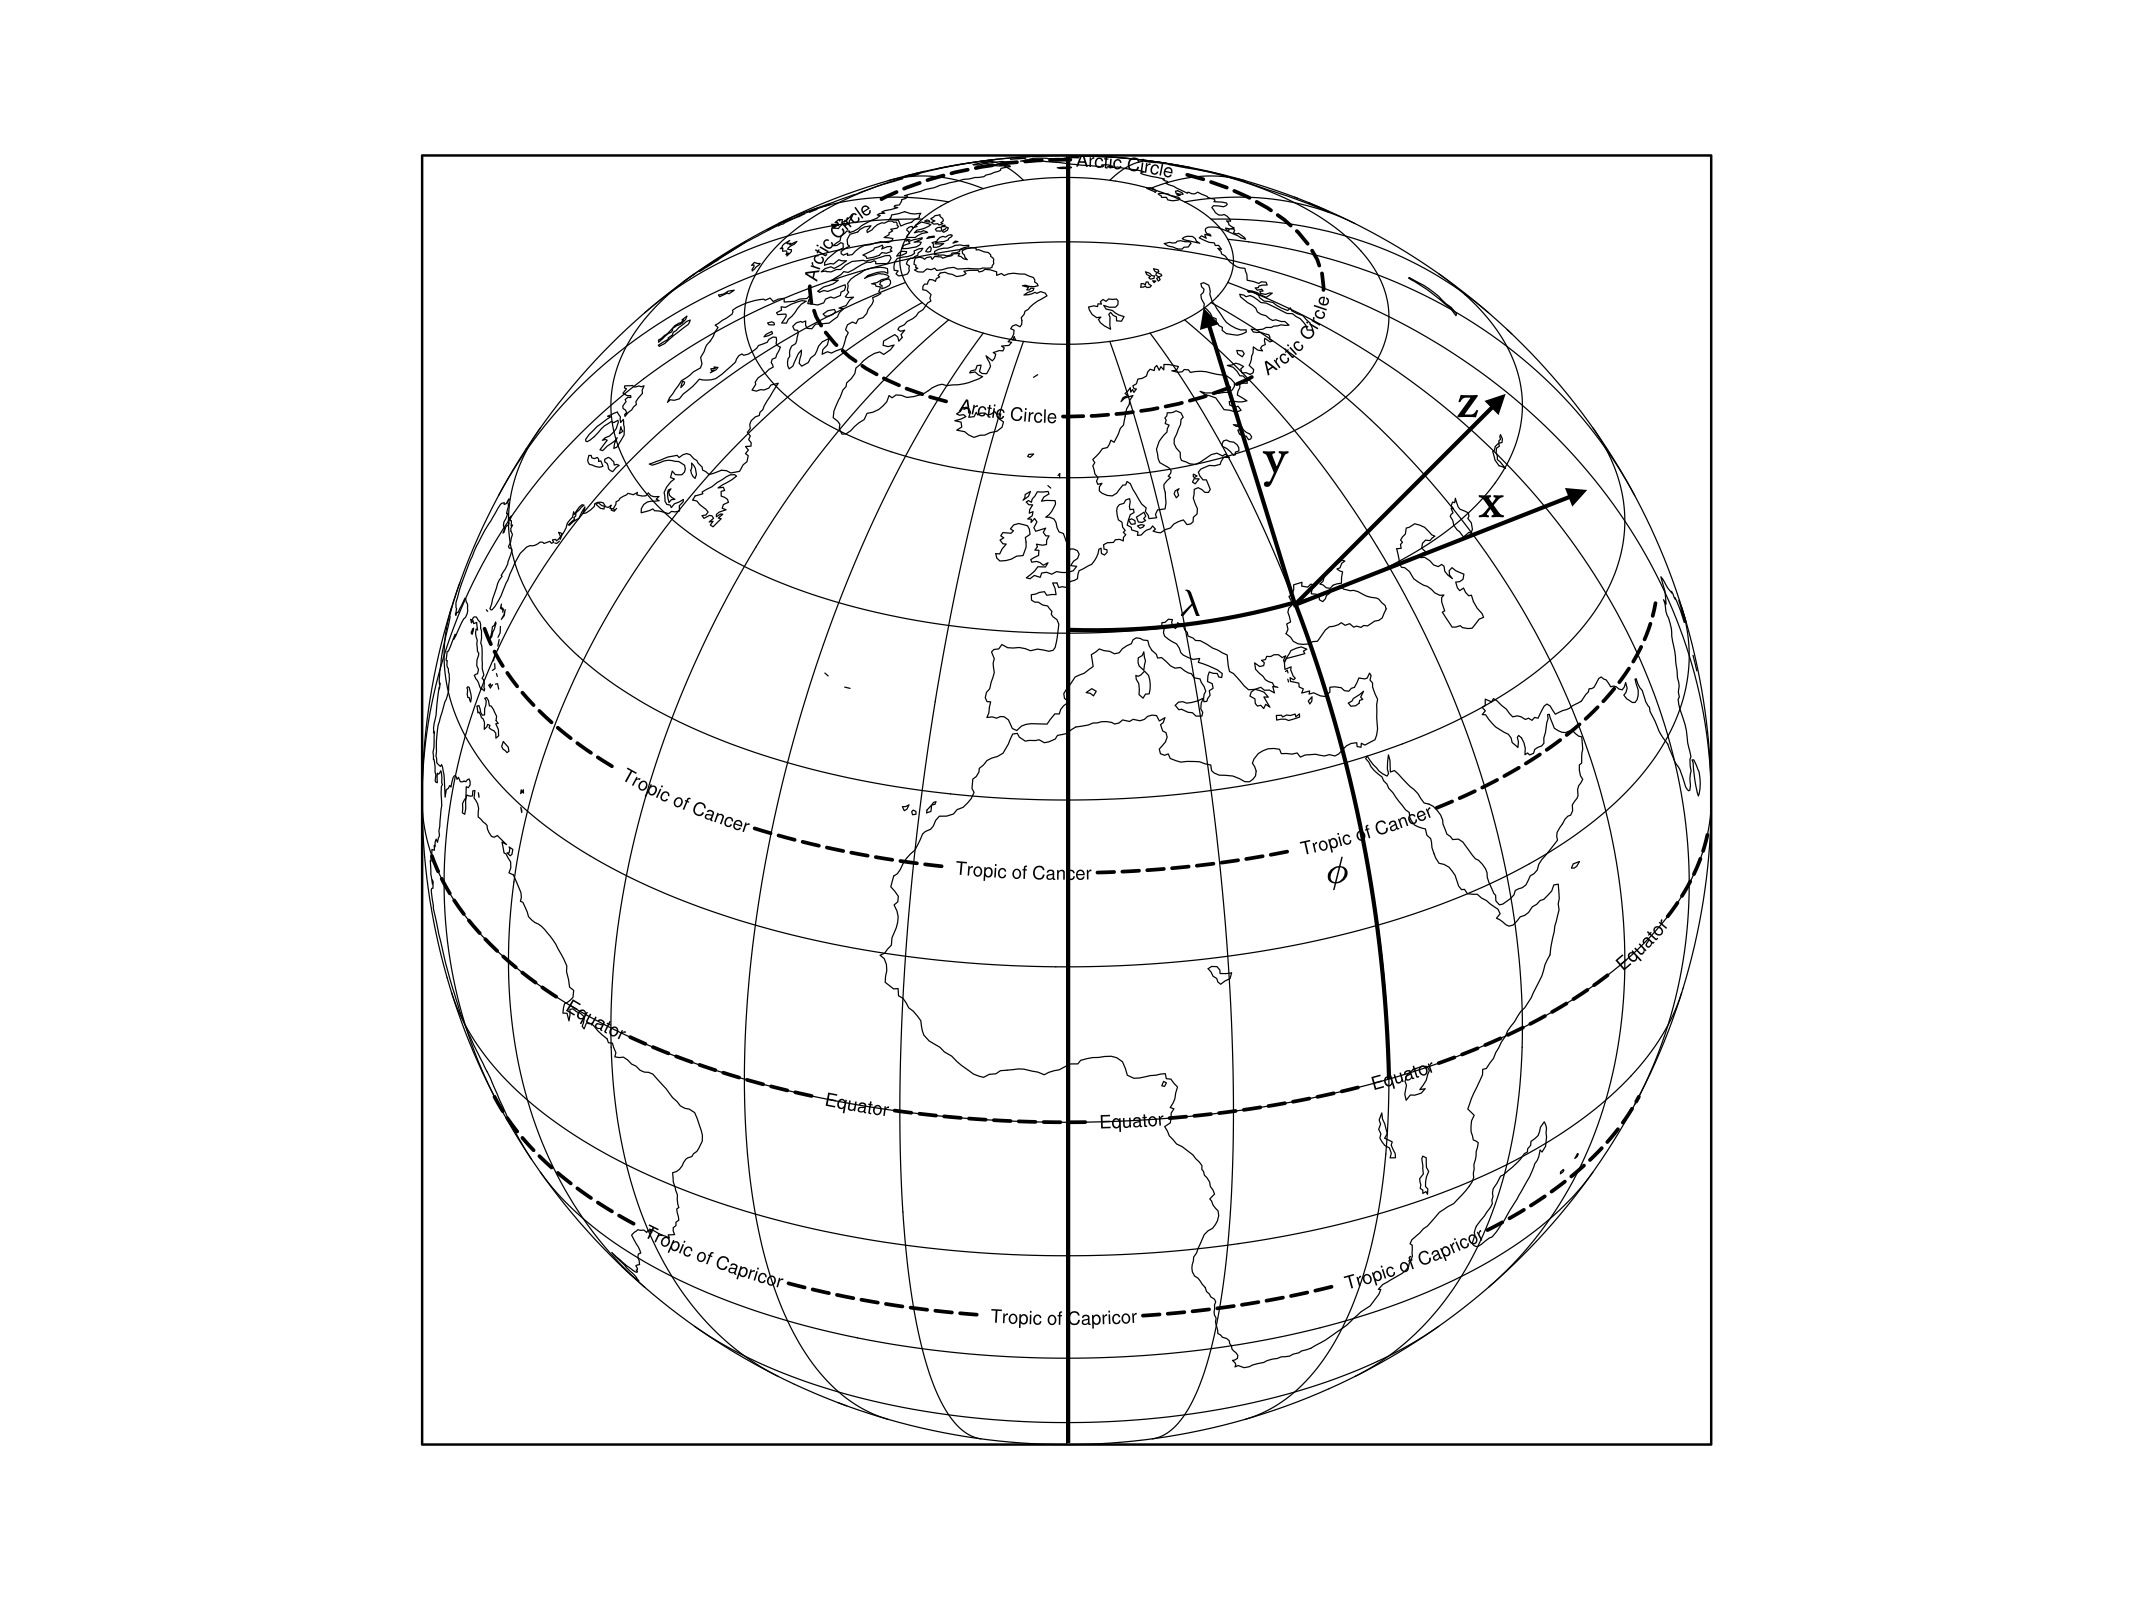
\includegraphics[width=0.8\textwidth]{figs/3d-coordinate-sys}
	\caption{3D Spherical coordinate system.}
	\label{fig:3d-coordinate-sys}
\end{figure}

\subsection{Rates of change of fluid properties over time: Eulerian vs Lagrangian description}\label{subsec:eulerian-lagrangian-derivative}

In fluid dynamics, there are two primary perspectives for describing the motion of fluids and their properties: the Eulerian and the Lagrangian.

The \textbf{Eulerian description} focuses on specific points in space through which the fluid flows.
Changes in fluid properties, such as velocity, temperature, or pressure, are observed at these fixed spatial locations over time.
This is analogous to standing on a bridge and watching water flow underneath.
This perspective is often used in large-scale atmospheric and oceanic studies.

In contrast, the \textbf{Lagrangian description} follows individual fluid parcels as they move through space and time.
It tracks changes in the properties experienced by these parcels.
This is akin to floating along with the current in a boat and observing changes in the surrounding environment.
This perspective is particularly useful when studying transport and mixing in fluids, such as pollutant dispersion or cloud formation.

The connection between these two perspectives is captured by the \textbf{advective derivative} - also know as \emph{material derivative} or
\emph{Lagrangian derivative} - which describes the rate of change of a property $\phi= \phi(\bm{x},t)$ as seen from the perspective of a moving fluid parcel.
It combines the local rate of change (Eulerian derivative) and the transport of the property due to the fluid motion (advection).
Mathematically, the advective derivative is expressed as:
\begin{equation}
	\materiald{\phi} = \frac{\partial \phi}{\partial t} + \bm{u} \cdot \nabla \phi
	\label{eq:material-derivative}
\end{equation}
where:
\begin{itemize}
	\item $\materiald{\phi}$ is the advective derivative, representing the total rate of change of $\phi$ in a moving frame;
	\item $\frac{\partial \phi}{\partial t}$ is the Eulerian derivative, capturing the local rate of change of $\phi$ at a fixed location;
	\item $\bm{u} \cdot \nabla \phi$ is the advection term, representing the transport of $\phi$ by the fluid velocity $\bm{u}$.
\end{itemize}
\begin{pf}{
		To compute the total rate of change of a fluid property $\phi$ we have to consider it is
		evolving both in time $t$ and in space $\bm{x}$ (the fluid is moving), therefore
		\begin{equation}
			\frac{\partial \phi}{\partial t} + \frac{\partial x}{\partial t}\frac{\partial \phi}{\partial x} + \frac{\partial y}{\partial t}\frac{\partial \phi}{\partial y}+\frac{\partial z}{\partial t}\frac{\partial \phi}{\partial z} = \frac{\partial \phi}{\partial t} + \bm{u}\cdot\nabla\phi
			\label{eq:total-derivative}
		\end{equation}
		where we have recovered \eq{\ref{eq:material-derivative}}.
	}
\end{pf}


\section{Primitive equations}
\label{sec:primitive-equations}

The motion of a physical system is governed by conservation laws: conservation of momentum (\eq{\ref{eq:momentum-eq-atm}}),
mass (\eq{\ref{eq:continuity-equation}}) and energy (\eq{\ref{eq:thermal-energy-conservation}}).
The conservation of momentum equation will identify the forces acting on the system.
The conservation of energy will identify the processes capable of changing the energy of the system, i.e.~thermodynamical processes.

\subsection{Momentum equation}
\label{subsec:momentum-equation-atm}

The first set of fundamental equations that we encounter is the conservation of momentum, which, for a geophysical
fluid correspond to the \textbf{Navier-Stokes equations}.
The Navier-Stokes equations describe the motion of fluid substances like air and water.
They account for forces due to pressure, viscosity, and external forces such as gravity.
This set of equations is key to understanding how winds, ocean currents, and other flows evolve due to internal and external forces.
In the rotating reference frame described in~\secref{\ref{subsec:spherical-coordinate-systems}}
the aforementioned governing equations, written along three coordinates longitude $\lambda$, latitude $\phi$
and vertical direction $z$, read:
\begin{subequations}
	\begin{align}
		\materiald{u} -\frac{uv \tan{\phi}}{r} +  \frac{uw}{r}  & = -\frac{1}{\rho r \cos{\phi}}\frac{\partial p}{\partial \lambda} + fv - \hat{f}w + F_\lambda \\
		\materiald{v} -\frac{u^2 \tan{\phi}}{r} +  \frac{vw}{r} & = -\frac{1}{\rho r }\frac{\partial p}{\partial \phi} - fu  + F_\phi                           \\
		\materiald{w} -\frac{u^2+v^2}{r}                        & = -\frac{1}{\rho }\frac{\partial p}{\partial z} -g +\hat{f}u + F_z
	\end{align}
	\label{eq:momentum-eq-atm}
\end{subequations}
where $ \vec{u} = (u, v, w)$ is the fluid's velocity along the $\lambda, \phi, z$ directions
\begin{subequations}
	\begin{align}
		u & = a\cos{\phi\frac{\partial \lambda}{\partial t}} \\
		v & = a \frac{\partial \phi}{\partial t}             \\
		w & = \frac{\partial z}{\partial t}
	\end{align}
	\label{eq:velocity-spherical-coord}
\end{subequations}
and the advective derivative~(\eq{\ref{eq:material-derivative}}) in spherical coordinates reads:
\begin{equation}
	\materiald{} = \frac{\partial }{\partial t} + \frac{u}{a\cos{\phi}}\frac{\partial }{\partial \lambda} +\frac{v}{a}\frac{\partial }{\partial \phi} + w\frac{\partial }{\partial z} \, \cdot
	\label{eq:advective-derivative-spherical}
\end{equation}


Because a is the Earth's mean radius, z is height above the Earth's surface, and
$r = a + z$, it follows that for the atmospheric heights under consideration, $z \ll a$ and
$r$ generally can be replaced by $a$. This is known as the \emph{shallowness
	approximation}, because it results from the relatively shallow depth of the atmosphere
compared to the Earth's radius.
Also, since in climate-oriented general circulation
models the motions of primary interest have characteristic horizontal space scales of
hundreds to thousands of \unit{\kilo\meter} and velocities on the order of \qty{10}{\meter\per\second}, we can simplify
\eq{\ref{eq:momentum-eq-atm}} further by eliminating several of the generally less-significant terms,
such as $\hat{f}w, \hat{f}u$ and $\frac{u^2+v^2}{r}$ by assuming $g$ is constant.
In this approximations~\eq{\ref{eq:momentum-eq-atm}} simplifies to~\citep{Washington2005}:
\begin{subequations}
	\begin{align}
		\materiald{u} - v\left(f +  \frac{u \tan{\phi}}{a}\right) & = -\frac{1}{ a \cos{\phi}}\frac{1}{\rho}\frac{\partial p}{\partial \lambda} + F_\lambda \label{eq:momentum-shallow-u} \\
		\materiald{v} + u\left( f + \frac{u \tan{\phi}}{a}\right) & = -\frac{1}{a}\frac{1}{\rho}\frac{\partial p}{\partial \phi}  + F_\phi   \label{eq:momentum-shallow-v}                \\
		\materiald{w}                                             & = -\frac{1}{\rho }\frac{\partial p}{\partial z} -g  + F_z  \, \cdot \label{eq:momentum-shallow-w}
	\end{align}
	\label{eq:momentum-eq-atm-shallow}
\end{subequations}

The second term on the left-hand side of~\eq{\ref{eq:momentum-shallow-u}} represents the Coriolis force and the centrifugal force in the rotating reference frame of the Earth.
$f$ is the Coriolis parameter, which depends on the latitude $\phi$ and is given by $f=2\Omega\sin\phi$.
The Coriolis force is proportional to the velocity and acts perpendicular to the motion of the fluid, deflecting the
fluid in different directions depending on the hemisphere.
Note that the Coriolis term arises due to the rotation of the Earth, which introduces an apparent force in a rotating reference frame.
This term depends explicitly on the latitude because of how the Earth's rotation affects the direction and magnitude of the Coriolis
effect at different points on the Earth's surface.
The Coriolis force explicitly depends on the sine of the latitude, as the projection of $\Omega$ onto the local horizontal plane is
$\Omega\sin\phi$ (the latitude $\phi$ determines the angle between the Earth's rotational axis and the local vertical.
$\Omega$ is the angular velocity vector of Earth's rotation, it points along the axis of rotation (towards the North Pole). At the Equator $\phi=0°$ the Coriolis effect is perpendicular to $\Omega$ and has a max horizontal effect. At the poles ($\phi=\pm 90°$) the effect aligns with $\Omega$, and only the vertical motion is affected.

On the right side of all the three equations~\ref{eq:momentum-eq-atm-shallow} we find the pressure gradient force in the
longitudinal (first) and latitudinal (second) directions, which drives fluid motion
due to differences in pressure.
The terms $F_{\lambda}$, $F_{\phi}$ and $F_{z}$ represent an \emph{additional force} term that could represent any other forcing acting on the fluid parcel in the longitudinal, latitudinal and vertical direction.
It might include friction, external forces, or any other model-specific forces not accounted for in the other terms.

The term $\frac{u\tan\phi}{a}$ present in~\eq{\ref{eq:momentum-shallow-u}} accounts for the centrifugal force resulting
from the Earth's rotation.
Here, $u$ is the east-west velocity, $\phi$ is the latitude, and $a$ is the Earth's radius.
The centrifugal force is stronger near the equator, and this term adjusts the Coriolis effect to account for that.
$\frac{\partial p}{\partial\lambda}$ indicates how pressure changes as you move longitudinally, i.e. east or west.
The term $a\cos\phi$ accounts for the spherical geometry of the Earth and the fact that distances between lines of longitude vary with latitude (they are widest at the Equator and shrink towards the poles). This term describes the acceleration due to the horizontal pressure gradient in the longitudinal direction, with the pressure gradient force causing flow from regions of higher to lower pressure.

The term $\frac{v\tan\phi}{a}$ in~\eq{\ref{eq:momentum-shallow-v}} is the centrifugal force term in the north-south direction,
considering Earth's curvature.
$\frac{p}{\phi}$ represents the pressure gradient in the latitude direction, and it drives motion from high to low pressure.

As for the vertical direction,~\eq{\ref{eq:momentum-shallow-w}}, the the vertical component of the Coriolis force is negligible
because $\Omega$ is nearly parallel to the vertical axis in most regions.
In rotating systems like the atmosphere or oceans, vertical Coriolis terms are often ignored.
Gravity acts downward and opposes the upward motion.


The system of equations~\ref{eq:primitive-equations} is not closed: there are 5 variables but only 3 equations.
Therefore additional relationships need to be found to close the system.
As we shall now see, the fundamental conservation laws allow to do that.

\subsection{Mass conservation}\label{subsec:mass-conservation}

The mass of the fluid must be conserved locally, because there are now sinks or sources in the atmosphere itself, so we want to write the mass of a volume of
atmosphere fixed in space as
\[
	M = \int_V  \rho \,dV
\]
the mass in the volume can only change if there is a flux of mass at surface \(S\),
\[
	\frac{\partial }{\partial t} \int_V  \rho \,dV = -\int_S \rho \, \bm{u}\cdot n \, dS
\]
using the divergence theorem however we have
\[
	\frac{\partial }{\partial t} \int_V  \rho \,dV = -\int_V \nabla\cdot(\rho\bm{u}) \,dV
\]
because the volume is not changing with time we can bring the derivative inside the integral and we get
\[
	\int_V  \frac{\partial \rho}{\partial t}+\nabla\cdot(\rho\bm{u}) \,dV = 0
\]
but the volume is arbitrary, so it must be that
\begin{equation}
	\frac{\partial \rho}{\partial t}+\nabla\cdot(\rho\bm{u}) = 0
	\label{eq:continuity-equation}
\end{equation}
is valid locally.

The \textbf{conservation of mass} or \textbf{continuity equation}~\ref{eq:continuity-equation} ensures that the mass is
conserved in the system expresses how the density of air or water changes over time due to processes like flow and diffusion.
In particular, $\nabla\cdot(\rho\vec{v})$ represents the divergence of the mass flux, which accounts for the movement of the mass.

\subsection{First law of thermodynamics}\label{subsec:thermal-energy-conservation}
We have still at our disposal the conservation of thermodynamical energy and so we can also use the first law of thermodynamics for a gas,
that is a statement of internal energy, where $c_v$ is the specific heat for air at constant volume and $T$ is the temperature in Kelvins:
\begin{equation}
	c_v\materiald{T} = -p\materiald{}\left(\frac{1}{\rho}\right)+ Q
	\label{eq:thermal-energy-conservation}
\end{equation}
where we included the temperature and heating/cooling term \(Q\) (which is the net heat gain or loss to the external sources, for example the solar insolation, heating or cooling due to long wave radiation, latent heating due to condansation of water vapor into liquid water, and sensible heating due to conduction and convection).
The state variables are then linked by the~\textbf{equation of state} for an ideal gas
\begin{equation}
	p = \rho R T
	\label{eq:ideal-atm-equation-state}
\end{equation}
where \(R\) is the gas constant for dry air.

We can now use~\ref{eq:ideal-atm-equation-state} to write the energy equation~\ref{eq:thermal-energy-conservation}
(or the temperature equation) in a different form,
\[
	c_v\materiald{T} = -p\materiald{}\left(\frac{R T}{p}\right)+ Q = -R\materiald{T} + \frac{RT}{p}\materiald{p} + Q
\]
or (since for an ideal gas $c_p = c_v +R$),
\[
	c_p\materiald{T}  - \frac{1}{\rho}\materiald{p} = Q
\]
For many purpose atmospheric and oceanic motions can be considered essentially adiabatic. However, for climate studies, the assumption of exclusively adiabatic processes is not appropriate since the amount of heat added or lost to a unit volume of air or water over a long period of time can be substantial. For adiabatic processes \(Q=0\):
\[
	\begin{aligned}
		 & c_p\materiald{T}  - \frac{1}{\rho}\materiald{p} = 0        \\
		 & \frac{c_p}{T}\materiald{T} -\frac{R}{p}\materiald{p} = 0   \\
		 & \materiald{}\log{T} - \frac{R}{c_p}\materiald{}\log{p} = 0
	\end{aligned}
\]
integrating it we get
\[\log{T/T_0} - \log{\left(\frac{p}{p_0}\right)^{R/c_p}} = \text{const}\]
or
\begin{equation}
	\frac{T}{T_0}\left(\frac{p_0}{p}\right)^{R/c_p} = \text{const}
	\label{eq:T-T0-adiabatic}
\end{equation}
so the quantity, known as \emph{potential temperature}
\begin{equation}
	\theta = T\left(\frac{p_0}{p}\right)^{R/c_p}
	\label{eq:potential-temperature-def}
\end{equation}
is conserved in adiabatic processes and the thermodynamics equation can be written as
\begin{equation}
	\materiald{\theta} = Q \, \cdot
	\label{eq:potential-temp-rate}
\end{equation}
\eq{\ref{eq:potential-temp-rate}} quantifies the rate of change of a scalar quantity
(like temperature or moisture) for a fluid parcel moving through space.
The source term $Q$ could represent a source of energy or mass, such as heat from the sun or moisture added by evaporation.
In the context of a weather or climate model, this would represent how temperature (or another variable)
changes as the air parcel moves and as energy is gained or lost.

\subsection{Hydrostatic balance}\label{subsec:hydrostatic-balance}
Under the action of gravity the vertical component of the pressure
gradient force balances the action of gravity, resulting in very small
vertical acceleration
\[
	\frac{\partial p}{\partial z} =  -g \rho
\]
then if we take the vertical derivative of~\eq{\ref{eq:T-T0-adiabatic}}
\[
	\frac{1}{T_0}\frac{d T}{dz}\left(\frac{p_0}{p}\right)^{R/c_p} -\frac{p_0}{p^2}\frac{R}{c_p}\frac{T}{T_0}\left(\frac{p_0}{p}\right)^{R/c_p-1}\frac{d p}{dz} = 0
\]
simplifying
\[
	\frac{d T}{dz} -\frac{p_0}{p^2}\frac{R}{c_p}T\left(\frac{p_0}{p}\right)^{-1}\frac{d p}{dz} = 0
\]
or
\[
	\frac{d T}{dz} -\frac{1}{p}\frac{R}{c_p}T\frac{d p}{dz} = \frac{d T}{dz} +g\rho\frac{1}{p}\frac{R}{c_p}T = 0
\]
but using the equation of state~\ref{eq:ideal-atm-equation-state}
\begin{equation}
	\frac{d T}{dz} = -\frac{g}{c_p}
	\label{eq:adiabatic-lapse-rate}
\end{equation}
yields the temperature gradient with height under adiabatic
conditions and when the hydrostatic balance is valid.
This is known as the \emph{adiabatic lapse rate}; for sea-level dry air at \qty{0}{\celsius} $c_p \simeq \qty{1000}{\joule \per \kilo\gram \per \kelvin}$, thus we
get an estimate of it
\begin{equation}
	\frac{g}{c_p} = \qty{10}{\celsius \per \kilo\meter} \, \cdot
	\label{eq:adiabatic-lapse-rate-value}
\end{equation}
Under this assumptions there is a linear drop in temperature with height.

If we integrate over height $z$, assuming isothermal atmosphere, we get an exponential density $\rho$ and pressure $p$ decay
with height:
\begin{equation}
	p(z)=p_0 \exp{\left(- \frac{RT}{g}z\right)} \, \cdot
	\label{eq:pressure-profile-isothermal-atm}
\end{equation}


\subsection{Geostrophic balance}\label{subsec:geostrophic-balance}
Geostrophic balance is the balance between Coriolis Force and the horizontal component of the pressure gradient force.
Under this assumptions, equations~\ref{eq:momentum-shallow-u} and~\ref{eq:momentum-shallow-v} become, respectively
\citep{Gill1982}:
\begin{align}
	f v & = \frac{1}{\rho} \partialx{p}                 \\
	f u & = - \frac{1}{\rho} \partialy{p} \totald{f}{x}
\end{align}

\begin{figure}
	\centering
	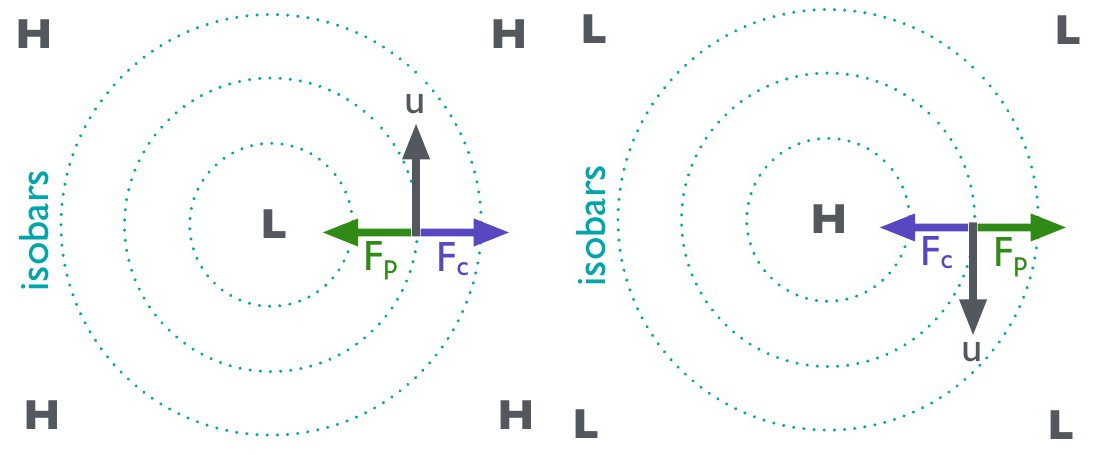
\includegraphics[width=0.9\textwidth]{figs/geostrophic-balance}
	\caption{
		Geostrophic winds follow a counterclockwise path in the Northern Hemisphere (and a clockwise path in the Southern Hemisphere) along the isobars of low pressure cells (cyclones).
		Geostrophic winds follow a a clockwise path in the Northern Hemisphere (and a counterclockwise path in the Southern Hemisphere) along the isobars of high pressure cells (anti-cyclones).
		Taken from \href{http://integrate.mutz.science}{INTEGRATE Teaching Package}.}
	\label{fig:geostrophic-balance}
\end{figure}
The pressure gradient force (PGF) pushes air or water from high pressure to low pressure. The Coriolis force deflects the motion to the right in the Northern Hemisphere and to the left in the Southern Hemisphere. In geostrophic balance, these forces are equal in magnitude and opposite in direction. The geostrophic balance assumes the flow is steady and does not accelerate, so it neglects the effects of inertia. This balance is most accurate for large-scale motions (e.g., planetary or synoptic scales) where friction and other forces are negligible. Vertical motions are typically much smaller than horizontal motions and are neglected in geostrophic balance.
\begin{equation}
	\vec{v} = \unitv{k} \times \frac{1}{f \rho} \grad p
\end{equation}
In geostrophic balance:
\begin{itemize}
	\item Air or water flows parallel to the isobars (lines of constant pressure) or contours of constant geopotential height.
	\item The speed of the geostrophic flow increases with stronger pressure gradients (closer isobars).
\end{itemize}
However, on small scales (e.g., tornadoes, boundary layers), friction and other forces become important, so geostrophic balance is less accurate. Near the Equator, The Coriolis parameter ($f$) approaches zero, making the geostrophic balance invalid.

%\subsubsection{Advective derivative in rotating coordinates.}
%A vector in spherical coordinates is:
%\[
%	\bm{u} = u \unitv{\imath} + v \unitv{\jmath}+ w \unitv{k}
%\]
%but the unit vectors move in a rotating frame, so the advective derivative of a vector is given by:
%\begin{equation}
%	\materiald{\vec{u}}=\materiald{u}\unitv{\imath}+\materiald{v}\unitv{\jmath}+\frac{Dw}{Dt}\unitv{k}+u\frac{D\unitv{\imath}}{Dt}+v\frac{D\unitv{\jmath}}{Dt}+w\frac{D\unitv{k}}{Dt}
%	\label{eq:adv-derivative-rotating-frame}
%\end{equation}

\subsubsection{Coriolis Factors}\label{subsubsec:coriolis-factors}
The Coriolis forces derives from the conservation of angular momentum.
\[\materiald{}\left(R_A(\Omega R_A+u)\right)=0\]
or
\[2\Omega R_A\frac{dR_A}{dt}+u\frac{dR_A}{dt}+R_A\materiald{u}=0\]
rearraging
\[\materiald{u}=(2\Omega R_A+u)\frac{dR_A}{dt}\]
\begin{figure}[h!]
	\centering
	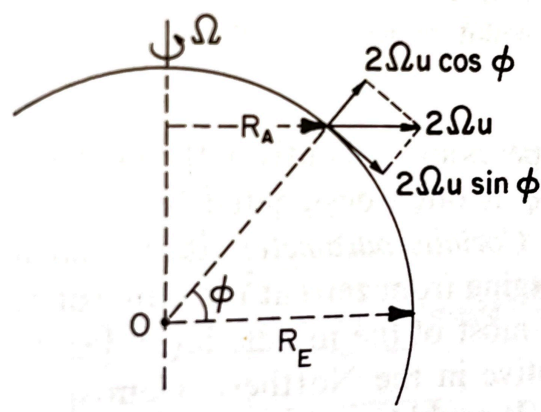
\includegraphics[width=0.35\linewidth]{uploads/Screenshot 2024-11-21 164025.png}
	\caption{Coriolis factors}
	\label{fig:coriolis-factors}
\end{figure}
The Coriolis components then are $2\Omega\sin\phi$ and $2\Omega\cos\phi$. For the horizontal and vertical components respectively:
$f=2\Omega\sin\phi$.

\subsection{The full set of governing equations for the atmosphere}
\label{subsec:governing-eqs-atm}

The full set of governing equations (Equations~\ref{eq:momentum-eq-atm-shallow},~\ref{eq:potential-temp-rate},~\ref{eq:continuity-equation} and~\ref{eq:ideal-atm-equation-state})
under the approximations described in~\secref{\ref{subsec:momentum-equation-atm}}
(shallowness condition, neglect of $w$ terms) can now be written as\footnote{The hydrostatic condition is not enforced
	for the system~\ref{eq:primitive-equations-full}.}:
\begin{subequations}
	\begin{align}
		 & \materiald{u} - v\left(f +  \frac{u \tan{\phi}}{a}\right)  = -\frac{1}{ a \cos{\phi}}\frac{1}{\rho}\frac{\partial p}{\partial \lambda}   + F_\lambda                                                      \\
		 & \materiald{v} + u\left( f + \frac{u \tan{\phi}}{a}\right)  = -\frac{1}{a}\frac{1}{\rho}\frac{\partial p}{\partial \phi}  + F_\phi                                                                         \\
		 & \materiald{w}  = -\frac{1}{\rho }\frac{\partial p}{\partial z} -g  + F_z \label{Eq:PrimEq}                                                                                                                \\
		 & \materiald{\theta} = Q                                                                                                                                                                                    \\
		 & \frac{\partial \rho}{\partial t}+\frac{1}{a\cos{\phi}}\left[ \frac{\partial }{\partial \lambda}(\rho u) + \frac{\partial }{\partial \phi}(rv\cos{\phi} )\right] +\frac{\partial }{\partial z}(\rho w) = 0 \\
		 & p = \rho R T
	\end{align}
	\label{eq:primitive-equations-full}
\end{subequations}
where we have expanded the divergence in spherical coordinates (see~Appendix~\ref{subsec:divergence}.).

These equations are still not closed because we will need to express the heating/cooling term \(Q\) and the friction terms \(F\)
as a function of the state variables.
This will require a theory of the processes that drive them.
Where \(R= \qty{287}{\joule \per\kilo\gram \per \kelvin}\) is the gas constant for dry air and
\(c_p \simeq \qty{1.005}{\joule \per \gram \per \kelvin}\) is the specific heat at constant pressure, \(c_v = \qty{0.718}{\joule \per \gram \per \kelvin}\) is the specific heat at constant volume, \(\kappa = \frac{R}{c_p}\) and \(\gamma=c_p/c_v\) is their ratio.

\subsection{$\beta$-plane approximation}
\label{subsec:beta-plane-primitive}

It can be convenient to shift the coordinate system when the latitudinal extent of motion is small relative to motion parameters expressed in adimensional numbers. In such cases, a tangent coordinate system is applied at a specific latitude \(\phi_0\), resulting in a Cartesian \(\beta\)-plane with zonal and meridional coordinates \((x, y)\).

On the \(\beta\)-plane, the planetary vorticity (see \eq{\ref{}}) \(f\) is linearized as \(f = f_0 + \beta y\), where \(\beta = \frac{\partial f}{\partial y}(\phi_0)\). The northward displacement \(y = a(\phi - \phi_0)\) represents deviation from the reference latitude.

This approximation simplifies geophysical fluid dynamics equations by neglecting rotation, sphericity, and certain meridional coordinates.
The equations~\ref{eq:primitive-equations-full} projected onto the \(\beta\)-plane simplify to
\begin{align}
	 & \materiald{u} - f v  = -\frac{1}{\rho}\frac{\partial p}{\partial x}   + F_x \\
	 & \materiald{v} + f u = -\frac{1}{\rho}\frac{\partial p}{\partial y}  + F_y   \\
	 & \materiald{w}  = -\frac{1}{\rho }\frac{\partial p}{\partial z} -g  + F_z    \\
	 & \materiald{\theta} = Q                                                      \\
	 & \frac{\partial \rho}{\partial t}+\nabla\cdot(\rho\bm{u}) = 0                \\
	 & p = \rho R T \, .
\end{align}


\section{Linear solutions to the primitive equations}\label{sec:linear-solutions}
We look for solution that describe small oscillation away from a basic state, in this case assumed in hydrostatic balance with constant wind of velocity $u$, and I'm looking at deviation from this basic state:
\begin{equation}
	\frac{\partial p_0}{\partial z}=-g\rho_0=-\frac{gp_0}{RT_0}
\end{equation}
With the further assumption of isotherm atmosphere we can integrate to get:
\begin{equation}
	p_0(z)=p_R \exp{(-z/H)}
\end{equation}
and $H=\frac{RT_0}{g}$ is the scale height.


As we have seen, the primitive equations are a system of nonlinear partial differential equations governing fluid motion on a rotating sphere. These include momentum equations, continuity (mass conservation), thermodynamic equations and the equation of state. Since solving the full nonlinear system is often impractical, the system is linearized to analyze small deviations (or perturbations) from a reference state (steady flow or a state of rest). Assume the flow can be separated into a basic state and a perturbation:
\begin{align*}
	u=u_0+u'                \\
	v=v_0+v'                \\
	\theta=\theta_0+\theta' \\
	p=p_0+p'
\end{align*}
The resulting linearized primitive equations describe how perturbations evolve over time and space (linear equations are obtained for the prime variables neglecting all terms quadratic in perturbation).
For instance, the pressure gradient becomes:
\begin{equation}
	\frac{1}{\rho_0+\rho'}\nabla(p_0+p')+g\unitv{k}\approx\frac{1}{\rho_0+\rho'}\nabla p'+g\unitv{k}=\frac{1}{\rho_0}\frac{1}{1+\frac{\rho'}{\rho_0}}\nabla p'+g\unitv{k}=\frac{1}{\rho_0}\nabla p'+g\unitv{k}
\end{equation}
and the potential temperature:
$$
	\theta=T\left(\frac{p_R}{p}\right)^k=\frac{p_R^k}{R}\frac{p^{1-k}}{\rho}\approx\theta_0\left[1+\frac{1}{\gamma}\left(\frac{p'}{p_0}\right)-\frac{\rho'}{\rho_0}\right]
$$
hence,
\begin{equation}
	\frac{\theta'}{\theta_0}=\frac{1}{\gamma}\frac{p'}{p_0}-\frac{\rho'}{\rho_0}
\end{equation}
with $\gamma=\frac{c_p}{c_v}$, $k=\frac{R}{c_v}$, $R=c_p-c_v$.

\subsection{Waves}
The linearized system often supports wave-like solutions. These solutions arise naturally due to the restoring forces in the equations, such as:
\begin{itemize}
	\item Pressure gradient drives the oscillations through compressibility or buoyancy
	\item Coriolis force introduces rotational effects leading to inertial and planetary waves
	\item Gravity acts as a restoring force for vertical displacement, driving internal gravity waves.
\end{itemize}

We take the equations for perturbation:
\begin{align*}
	\frac{\partial u}{\partial t}+U\frac{\partial u}{\partial x}+\frac{1}{\rho_0}\frac{\partial p}{\partial x}=0                                                              \\
	\frac{\partial w}{\partial t}+U\frac{\partial w}{\partial x}+\frac{1}{\rho_0}\frac{\partial p}{\partial z}+g\frac{\rho}{\rho_0}=0                                         \\
	\frac{\partial\rho}{\partial t}+U\frac{\partial\rho}{\partial x}+w\frac{\partial\rho_0}{\partial z}+\rho_0(\frac{\partial u}{\partial x}+\frac{\partial w}{\partial z})=0 \\
	\frac{\partial\theta}{\partial t}+U\frac{\partial\theta}{\partial x}+w\frac{\partial\theta_0}{\partial z}=0                                                               \\
	\frac{\theta}{\theta_0}+\frac{\rho}{\rho_0}+\frac{1}{\gamma}\frac{p}{p_0}=0
\end{align*}

%slides 24-29 LEC6 non le ha molto cagate
Basically to find solutions, assume the perturbations take the form of plane waves:
\[\bm{u'}(x,t)=\unitv{\bm{u}}e^{i(\bm{k}\cdot\bm{x}-\omega t)}\]
where $\bm{\unitv{u}}$ is the amplitude of the perturbation, $\bm{k}$ is the wavevector, $\omega$ the angular velocity. Substituing this kind of wave into the linearized equations leads to a dispersion relation, which relates $\omega$ to $\bm{k}$ and the physical parameters of the system (Coriolis, ...).
The perturbation equations link the restoring forces to wave properties:
\begin{enumerate}
	\item The momentum equations describe how velocity perturbations interact with pressure gradients and Coriolis forces.
	\item The continuity equation ensures mass conservation, connecting velocity and density perturbations.
	\item The thermodynamic equation relates temperature, pressure and density perturbations
\end{enumerate}
Imposing the hydrostatic approximation from the beginning would mean putting to zero from the start the time derivative of $w$ in the momentum equation in the vertical. This basically is equivalent to say that we are removing the explicit dependence of the vertical velocity on time and therefore we will get waves similar to the Boussinesq approximation. The hydrostatic approximation eliminates vertical propagating sound waves, but the Lamb waves still exists.


\section{Homogeneous flows}\label{sec:homogeneous-flows}

The motion of the atmosphere is most appropriately described by
three-dimensional equations that describes the horizontal and vertical
motion of the fluid, however a lot can be understood by considering a
simpler system that consider the motion of a free surface of a inviscid,
homogeneous and incompressible fluid. These equations are variously
referred to as one-level primitive equations or the \textit{shallow water
	equations}.
\begin{figure}
	\centering
	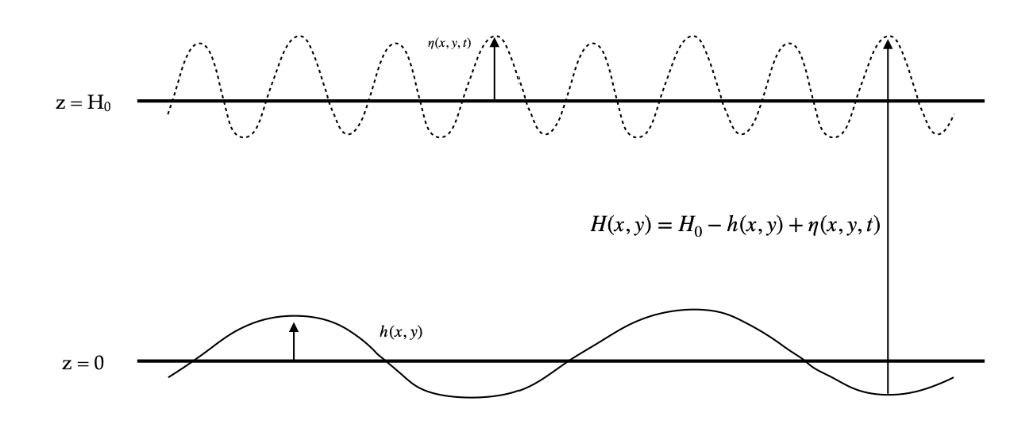
\includegraphics[width=0.7\textwidth]{uploads/image732864.png}
	\caption{Homogeneous flow}
	\label{fig:homogeneous-flow}
\end{figure}

The system is described in~\fig{\ref{fig:homogeneous-flow}}, it is an homogenous
layer of fluid covering the entire spherical planet. We have included a
bottom topography \(h(x,y)\) and a deformation of the free surface
\(\eta(x,y)\). The convention is such positive deformation of the
surface are increasing the depth of the fluid, whereas positive
deformation of the bottom are decreasing it.

We have introduced here cartesian coordinates \((x,y)\) such that
\(dx \approx a \cos\theta d \lambda\) and \(dy \approx a d\theta\), we
will also define \(f= 2\Omega \sin\theta\), then the incompressible
equations of motion can be written as

\[
	\begin{aligned}
		\frac{\partial u}{\partial t} & = -u \frac{\partial u}{\partial x} -v \frac{\partial u}{\partial y} + f v -\frac{1}{\rho}\frac{\partial p}{\partial x} \\
		\frac{\partial v}{\partial t} & = -u \frac{\partial v}{\partial x} -v \frac{\partial v}{\partial y} - f u -\frac{1}{\rho}\frac{\partial p}{\partial y} \\
		\frac{\partial w}{\partial t} & = -u \frac{\partial w}{\partial x} -v \frac{\partial w}{\partial y} + g -\frac{1}{\rho}\frac{\partial p}{\partial z}   \\
		                              & \frac{\partial u}{\partial x} + \frac{\partial v}{\partial y} + \frac{\partial w}{\partial z} = 0
	\end{aligned}
\]

If the aspect ratio \(\delta \approx H/L\) is small then hydrostatic
balance is maintained to order \(\delta^2\) and so

\[\frac{\partial p}{\partial z} = - \rho g + O(\delta^2)\]

because the density is constant we can integrate it from 0 to \(z\) and
get

\[p = -\rho g (H_0+ \eta -z) + p_0\]

where we have used the boundary condition at the top
\(p(x,y,H_0 +\eta) = p_0\).

The horizontal pressure gradients are independent of \(z\)

\[\begin{aligned}
		\frac{\partial p}{\partial x} = \rho g \frac{\partial \eta}{\partial x} \\
		\frac{\partial p}{\partial y} = \rho g \frac{\partial \eta}{\partial y}
	\end{aligned}\]

because the horizontal accelerations are independent of z, than also the
velocities are independent of z, if they are so at the beginning. This
is in fact a consequence of the Taylor-Proudman theorem applied to a
homogeneous fluid. We can then write the horizontal momentum equations

\[\begin{aligned}
		\frac{\partial u}{\partial t} & = -u \frac{\partial u}{\partial x} -v \frac{\partial u}{\partial y} + f v -g\frac{\partial \eta}{\partial x} \\
		\frac{\partial v}{\partial t} & = -u \frac{\partial v}{\partial x} -v \frac{\partial v}{\partial y} - f u -g\frac{\partial \eta}{\partial y} \\
	\end{aligned}\]

Because \(u\) and \(v\) are independent of \(z\) allows us to integrate
vertically the divergence equation from the surface \(h(x,y)\) to an
height \(z\)

\[w(x,y,z,t) = -z\left(\frac{\partial u}{\partial x} + \frac{\partial v}{\partial y}\right) + \omega(x,y,t)\]

The kinematic condition for the bottom can be written as

\[\materiald{}{(z-h)} = 0\]

or

\[w(x,y,h,t) =  u\frac{\partial h}{\partial x} + v\frac{\partial h}{\partial y}\]

so the function \(\omega\) is

\[\omega(x,y,t) = u\frac{\partial h}{\partial x} + v\frac{\partial h}{\partial y} + h \left(\frac{\partial u}{\partial x} + \frac{\partial v}{\partial y}\right)\]

then the vertical velocity can be written as

\[w(x,y,z,t) = (h-z)\left(\frac{\partial u}{\partial x} + \frac{\partial v}{\partial y}\right) + u\frac{\partial h}{\partial x} + v\frac{\partial h}{\partial y}\]

Using now the kinematic boundary condition at the top (\(z=H_0+\eta\))

\[w(x,y,H_0+\eta,t) = \left(\frac{\partial }{\partial t} + u\frac{\partial }{\partial x} + v\frac{\partial }{\partial y}\right)(H_0+\eta)\]

combining the last two equation we get an equation for the height

\[\frac{\partial \eta}{\partial t} + \frac{\partial }{\partial x}(H_0+\eta -h)u + \frac{\partial }{\partial y}(H_0+\eta -h)v = 0\]

and so we can now write the complete equations, introducing the total
depth of the fluid \(H=H_0+\eta -h\):

\[\begin{aligned}
		\frac{\partial u}{\partial t} & = -u \frac{\partial u}{\partial x} -v \frac{\partial u}{\partial y} + f v -g\frac{\partial H}{\partial x} \\
		\frac{\partial v}{\partial t} & = -u \frac{\partial v}{\partial x} -v \frac{\partial v}{\partial y} - f u -g\frac{\partial H}{\partial y} \\
		\frac{\partial H}{\partial t} & = - \frac{\partial (u H)}{\partial x} - \frac{\partial (v H)}{\partial y}                                 \\
	\end{aligned}\]
Linearizing around a state of rest, constant rotation:
\begin{align*}
	\frac{\partial u}{\partial t}-fv=-g\frac{\partial\eta}{\partial x} \\
	\frac{\partial v}{\partial t}+fv=-g\frac{\partial\eta}{\partial y} \\
	\frac{\partial\eta}{\partial t}=-H_0\left(\frac{\partial u}{\partial x}+\frac{\partial v}{\partial y}\right)
\end{align*}
the solutions are, respectively:
\begin{align*}
	u(x,y,t)=\text{Re}\left[\tilde{u}\sin(ly)e^{i(kx-\omega t)}\right] \\
	v(x,y,t)=\text{Re}\left[\tilde{v}\sin(ly)e^{i(kx-\omega t)}\right] \\
	\eta(x,y,t)=\text{Re}\left[\tilde{\eta}\sin(ly)e^{i(kx-\omega t)}\right]
\end{align*}
two modes\footnote{mode in this context refers to a specific solution or pattern of motion that satisfies the governing equations of the flow, under certain boudaries or initial conditions.}, a stationary mode and a gravity mode (Poincare' modes): $\omega=0$ and $\omega^2=f^2+gH_0(k^2+l^2)$


\subsection{\texorpdfstring{The vorticity equation on the
		\(\beta\)-plane}{The vorticity equation on the \textbackslash beta-plane}}\label{the-vorticity-equation-on-the-beta-plane}

The spherical geometry maybe cumbersome without adding much the
conceptual discussions, so it may be convenient to introduce Cartesian
coordinates \((x,y)\) such that \(dx \approx a \cos\theta d \lambda\)
and \(dy \approx a d\theta\), we will also define
\(f= 2\Omega \sin\theta\), then we obtain equation formally identical to
the Cartesian equation described previously

\[\begin{aligned}
		\frac{\partial u}{\partial t} & = -u \frac{\partial u}{\partial x} -v \frac{\partial u}{\partial y} + f v -g\frac{\partial \eta}{\partial x} \\
		\frac{\partial v}{\partial t} & = -u \frac{\partial v}{\partial x} -v \frac{\partial v}{\partial y} - f u -g\frac{\partial \eta}{\partial y} \\
		                              & \frac{\partial u}{\partial x}+\frac{\partial v}{\partial y} = 0                                              \\
	\end{aligned}\]

where we have kept the pressure terms, though they are zero in this case
($h$ is a constant) as a placeholder. In vector notation (all vectors are
two-dimensional)

\[\frac{\partial \bm{u}}{\partial t} = - (\bm{u} \cdot \nabla)\bm{u} - f(\unitv{k}\times \bm{u}) - \nabla \eta\]

using the vector identity\footnote{For a general vector $\bm{A}$: \[\frac{1}{2}\nabla(A\cdot A) = (A \cdot\nabla)A + A\times(\nabla\times A)\]}


\[\frac{1}{2}\nabla(\bm{u}\cdot \bm{u}) = (\bm{u} \cdot\nabla)\bm{u} + \bm{u}\times(\nabla\times \bm{u})\]
so substituting in the equation

\begin{equation}
	\frac{\partial \bm{u}}{\partial t} = -(\zeta + f) \unitv{k}\times \bm{u} -\nabla(\eta+\frac{1}{2}|\bm{u}^2|)
	\label{eq.21}
\end{equation}

(for 2-dimensional flows \(\nabla \times \bm{u} = \zeta \unitv{k}\)).

and to express more clearly the components

\[\begin{aligned}
		\frac{\partial u}{\partial t} & = (\zeta +f) v -\frac{\partial }{\partial x}(\eta+\frac{1}{2}|\bm{u}^2|)  \\
		\frac{\partial v}{\partial t} & = -(\zeta +f) u -\frac{\partial }{\partial y}(\eta+\frac{1}{2}|\bm{u}^2|)
	\end{aligned}\]

By taking the curl of eq.\ref{eq.21} we obtain an equation for the vorticity (as it will be discussed in Sec.\ref{Sec:models on the sphere}:

\[\begin{aligned}
		\frac{\partial \zeta}{\partial t} & = -\frac{\partial }{\partial x}(\zeta +f) u -\frac{\partial }{\partial y}(\zeta +f) v                                                                                  \\
		                                  & -\frac{\partial }{\partial x} \frac{\partial }{\partial y}(p+\frac{1}{2}|\bm{u}^2|) +\frac{\partial }{\partial y}\frac{\partial }{\partial x}(p+\frac{1}{2}|\bm{u}^2|) \\
		                                  & =  -\frac{\partial }{\partial x}(\zeta +f) u -\frac{\partial }{\partial y}(\zeta +f) v = -\bm{u}\cdot\nabla(\zeta +f)
	\end{aligned}\]

where we have used the non divergence condition
\(\frac{\partial u}{\partial x}+\frac{\partial v}{\partial y}=0\) in the
last step. Once again, this is the equation for the conservation of
total vorticity where we can see that the relative vorticity is a sort
of additional Coriolis effect (or alternatively that the Coriolis term
is a source of vorticity). Because of the $\beta$-plane $f=f_0+\beta y$:
\begin{equation}\label{Barotropic equation}
	\frac{\partial\zeta}{\partial t}=-u\frac{\partial\zeta}{\partial x}-v\frac{\partial\zeta}{\partial y}-\beta v
\end{equation}
that is the non-divergent barotropic vorticity equation. And the potential vorticity:
\begin{equation}\label{eq.potential vorticity}
	\materiald{}(\zeta +f)=0
\end{equation}

\(f= 2\Omega \sin(\theta)\) is the Coriolis coefficient, that is the
vertical component of the Earth planetary vorticity.

In the new coordinates \((x,y)\) for longitude and latitude, the
streamfunction and the vorticity then are

\[u=-\frac{\partial \psi}{\partial y}\qquad v=\frac{\partial \psi}{\partial x} \qquad
	\zeta = \frac{\partial x}{\partial x} -\frac{\partial u}{\partial y}=\nabla^2\psi\]

introducing the Jacobian operator

\[J(A,B) = \frac{\partial A}{\partial x}\frac{\partial B}{\partial y} - \frac{\partial A}{\partial y}\frac{\partial B}{\partial x}\]

we obtain a single equation for the streamfunction

\[\frac{\partial }{\partial t}\nabla^2\psi  + J(\psi, \nabla^2\psi +f_0 + \beta y) = 0\]
that represents the quasi-geostrophic potential vorticity.
Vorticity is a vertical component of the velocity, and appears coupled with $f$ , where $f$ is a propriety of the Earth and $\zeta$  is a propriety of the flow. Because the potential vorticity is conserved with the flow, if you have something at rest at the Equator and you move it Poleward, it acquire vorticity and starts speeding .


\section{Rossby waves}
Rossby waves or planetary waves are large-scale waves that arise in a rotating fluid, such as the Earth's atmosphere or oceans, due to the variation of the Coriolis parameter $f$ with latitude. In particular, they are caused by the $\beta$-effect, i.e. $\beta=\frac{\partial f}{\partial y}=\frac{2\Omega\cos\phi}{a}$. These waves typically have very large horizontal wavelengths and govern large-scale motions in the atmosphere and oceans, their restoring force is the variation of the Coriolis force with latitude. Rossby waves are much slower than other atmospheric or oceanic waves, such as gravity or sound waves.

Linearizing around a basic state $U$:
\begin{equation}
	\frac{\partial\zeta'}{\partial t}+U\frac{\partial\zeta'}{\partial x}-\beta\nu'=0
\end{equation}
the solutions are:
\begin{equation}
	\psi(x,y,t)=\text{Re}\left[\tilde{\psi}\sin(ly)e^{i(kx-\omega t)}\right]
\end{equation}
as\footnote{This will be understood after a reading of the Spectral Trasformation method in sec.\ref{sec:spectral method}.} $$\zeta=\nabla^2\psi=-(k^2+l^2)\psi$$
with $u=-il\psi$ and $\nu=ik\psi$
the dispertion relation is $$\omega=Uk-\frac{k\beta}{(k^2+l^2)}$$
\begin{figure}[htpb]
	\centering
	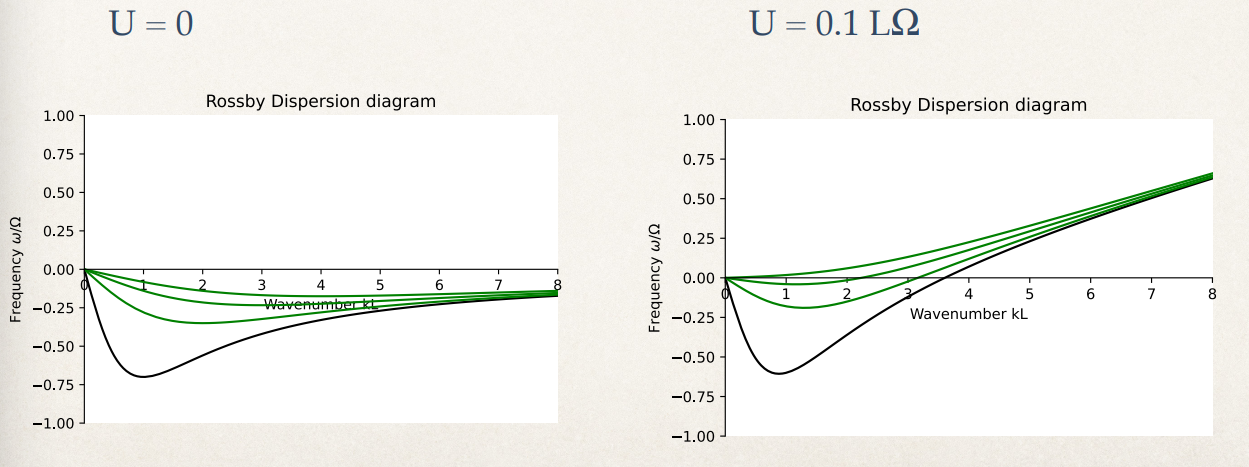
\includegraphics[width=0.5\linewidth]{uploads/Screenshot 2024-11-21 162828.png}
	\caption{Rossby waves}
	\label{fig:enter-label}
\end{figure}

\section{Fundamental processes}
Different climate models incorporate all the complex physical processes occurring in the climate system using a variety of methods. The dynamic involves interactions between motions, thermodynamics, and atmospheric water content.

\subsection{Radiation}
The radiation that heats and cools the climate system can be divided into two parts: solar radiation (shortwave) and terrestrial radiation (longwave).
All gases emit and absorb radiation, and each chemical element or combination of elements has a distinct spectrum indicating at which electromagnetic wavelengths its emissions occur. In some cases, the emission may be confined to narrow portions of the electromagnetic spectrum rather than being a smoothly varying function of wavelength. This phenomenon of distinct, discrete emission spectra results from the emission of radiation as an electron moves from one orbit around an atomic nucleus to another orbit closer to the nucleus. If the atom is excited by absorbing energy, then the electron can go to a higher (outer) discrete orbit.
As electrons return to the inner orbits, emission occurs in the ultraviolet part of the spectrum, producing the emission spectra. If electrons return to intermediate orbits instead of higher orbits, the emission is in the visible part of the spectrum; for the outer orbits, the emission is in the infrared.
So far we have discussed only the emission of energy from a gas, not the absorption of energy. Suppose radiational energy enters an atomic or molecular gas and is absorbed. In that case, it can increase the atomic or molecular energy levels by the same amount of energy involved in the emission. This absorption can be just as discrete or selective as the emission. Thus, if radiation entering a gas cannot excite the atoms or molecules in any energy form, then the radiational energy will not be absorbed or emitted in the gas.\\


In the Earth's atmosphere, ozone, carbon dioxide, and water vapor are very important triatomic molecules that both emit and absorb radiation in certain parts of the electromagnetic spectrum that affect the climate system.

\begin{figure}[htp!]
	\centering
	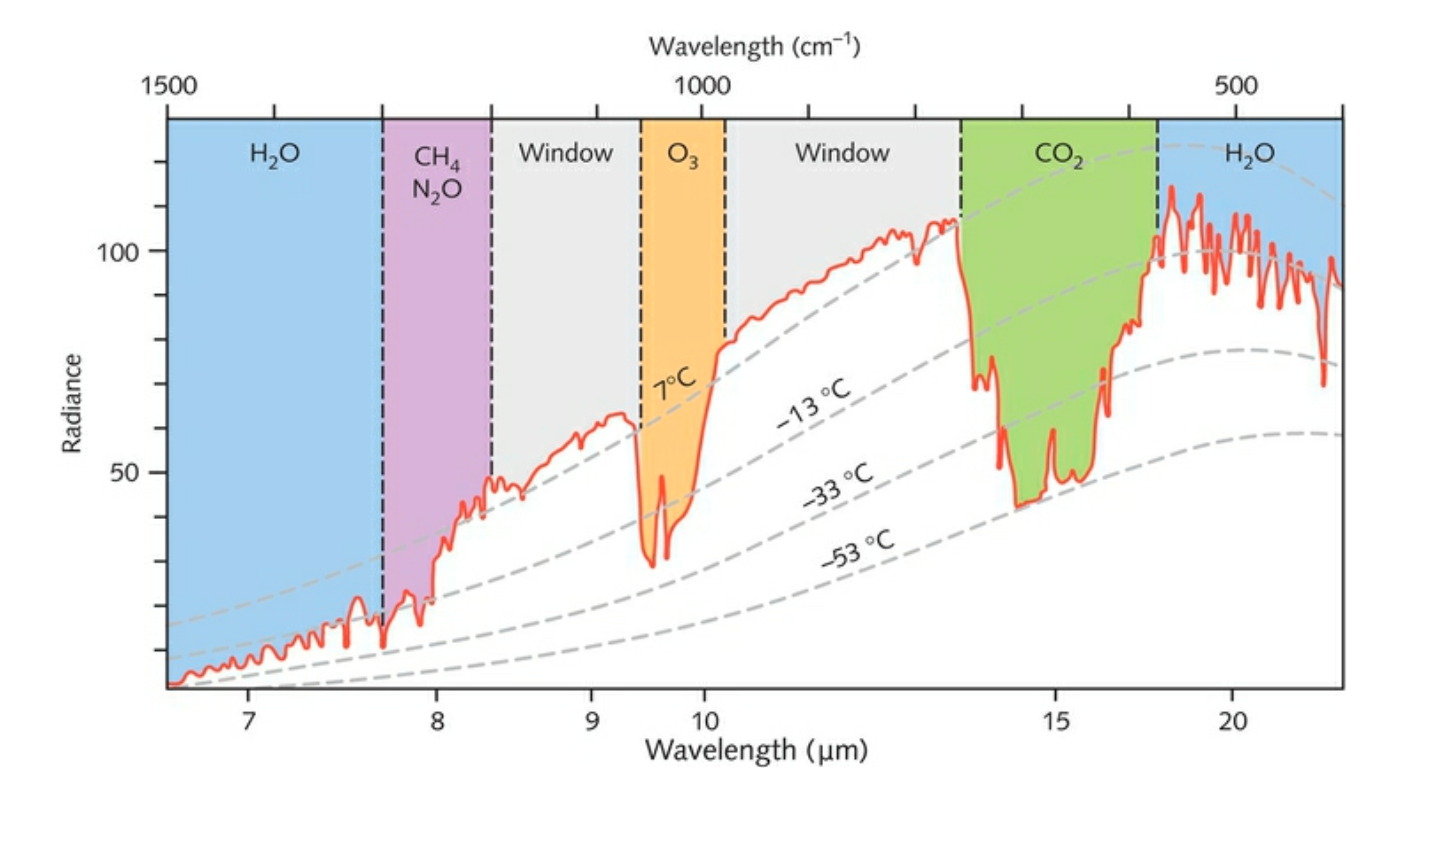
\includegraphics[width=0.5\linewidth]{uploads/image10.png}
	\caption{Earth's spectrum}
	\label{fig:2.7}
\end{figure}
As we can see in figure \ref{fig:2.7} ozone is a very strong absorber in the 9-10 $\mu$m region, carbon dioxide has absorption maxima in the 2, 3, 4, and 13-17 $\mu$m regions, and water vapor has several absorption regions in the 1-8 $\mu$m range and at wavelengths greater than 13 $\mu$m.

The radiational heating and cooling computation in climate models is usually done by calculating upward and downward fluxes through unit horizontal areas, considering the vertical distributions of temperature, water vapor, and other radiative absorbing gases such as carbon dioxide and ozone.

The blackbody radiation curve was determined theoretically by Max Planck in 1900. A result of Planck's equation is the earlier displacement law of Wien, that the wavelength of maximum intensity $\frac{2897.8}{T}$ where $T$ is the temperature of the blackbody.
For the Earth, the approximate global mean surface temperature is 293 K, which yields a maximum intensity near 9.9$\mu$m whereas for the sun the surface temperature is approximately $T$ = 6110K which yields a maximum intensity at 0.474$\mu$m The overlap of the blackbody radiation curves for the Earth and for the sun's radiation reaching the Earth is not great, and consequently solar and terrestrial radiation can be separated based on wavelength.

\begin{figure}[htp!]
	\centering
	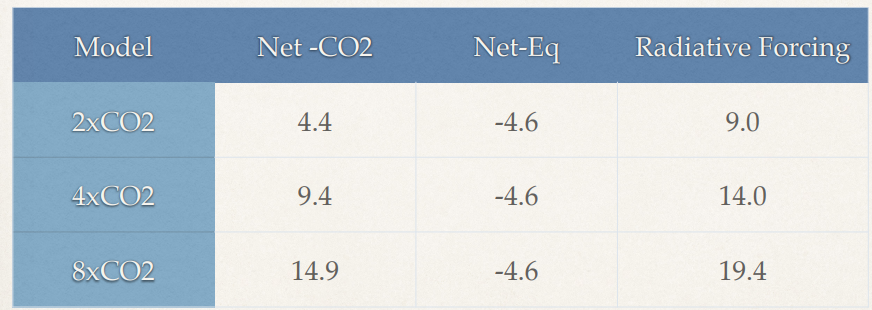
\includegraphics[width=0.4\linewidth]{uploads/image11.png}
	\caption{Black body curves for the solar radiation and the terrestrial radiation for the entire atmosphere and the first 11 km of the atmosphere}
	\label{fig:enter-label}
\end{figure}
Much of the fundamental physics governing radiation transfer is embodied in the following two laws:
\begin{itemize}
	\item Lambert's law, which provides a formulation for the decrease in intensity of radiation of a given wavelength as the radiation passes through a given amount of absorbing gas
	      $$\frac{d}{dz}[I]=-Ik\rho$$
	      where $k$ is the absorption coefficient (which tells us what kind of mass is preset), $\rho$ is the density of the layer, and $I$ is the radiance, defined as the energy per unit time per  unit area per unit solid angle $d\omega$

	\item Kirchhoff's law, states that there is a proportionality between radiative absorptivity and emissivity of a gas at the same temperature for any wavelength. A good absorber of radiation at some wavelength is also a good emitter of radiation at the same wavelength.

	      In particular, it is usually identified as \textit{absorptivity} the ratio of the amount of radiative energy absorbed to the total incident radiation, and \textit{emissivity} is the ratio of the emitted radiation to the maximum possible emitted radiation at the same temperature.
\end{itemize}


The \ref{fig:relat} shows the relationship between intensity from some given direction, unit solid angle $d\omega$, and the surface,
\begin{wrapfigure}{R}{0.38\textwidth}
	\begin{center}
		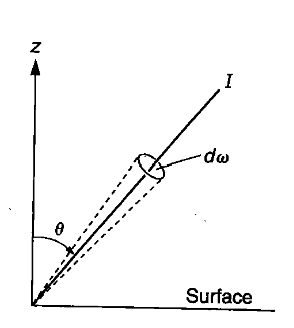
\includegraphics[width=0.22\textwidth]{uploads/imageIw.png}
	\end{center}
	\caption{Relationship between intensity}
	\label{fig:relat}
\end{wrapfigure}

such that integration over $\theta$ of the hemisphere above the horizontal surface yields the flux, $F$, arriving from all angles:
\begin{equation}
	F=\int(Icos\theta )\,d\omega
	\label{eq 2}
\end{equation}

Dividing \ref{eq 2} by $I$ and forming integrals over optical depth on either side yield
\[\int \frac{dI}{I} = - \int k \rho \, dz\]
which becomes
\[\ln \left( \frac{I}{I_0} \right) = - \int k \rho \, dz\]
upon integrating the left-hand side.
This can be written exponentially as
\[I = I_0 e^{-\chi}\]
\[\chi=\int k \rho \,dz \]
where $\chi$ is the optical depth or optical path length (rate at which the radiance is degraded, if you move upward, at a certain point you get zero because you have traveled enough to absorb all the radiation)  and
\[\tau = e^{-\chi}\]
is the frictional transmission, indicating the fraction of the original radiance that get transmitted to optical depth within attenuating gas. If $\chi=1$, then $\tau=0.37$ , which means the initial intensity $I$ is decreased by a factor of $0.63$ , for normal atmospheric conditions $\chi$ in typically much less than $1$.

For a blackbody, the emission is also described by Lambert's law with a different sign
\begin{equation}
	dI = B(T) k \rho \, dz
	\label{eq3}
\end{equation}

Integrating \ref{eq3} over a hemisphere, the Stefan-Boltzmann law is then obtained
\[\int_0^{2\pi} B(T) \cos \theta \, d\omega = \sigma T^4\]
or \[\pi B(T) = \sigma T^4\]

The change of radiance at a point z is made up of two fluxes
\[\frac{1}{\rho} \frac{dI}{dz} = -k (I - B(T))\] where $kI$ is the absorption and $kB(T)$ is the emission.
So the fractional absorption in a layer ($z$,$z_1$) is $$\tau(z, z_1) = \exp \left( - \int_{z_1}^z k \rho \, dz' \right)$$
\begin{figure}[htbp]
	\centering
	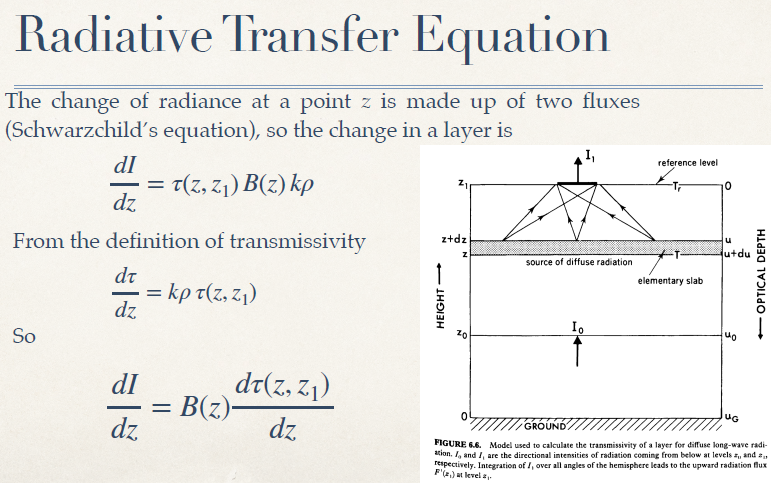
\includegraphics[width=0.35\linewidth]{uploads/16image.png}\quad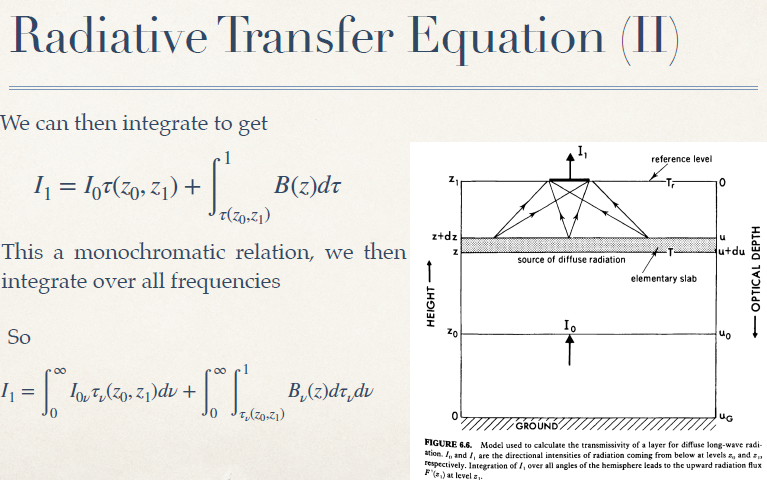
\includegraphics[width=0.35\linewidth]{uploads/17image.png}
	\caption{Non avevamo voglia di scriverli}
	\label{fig:enter-label}
\end{figure}




\begin{figure}[htpb]
	\centering
	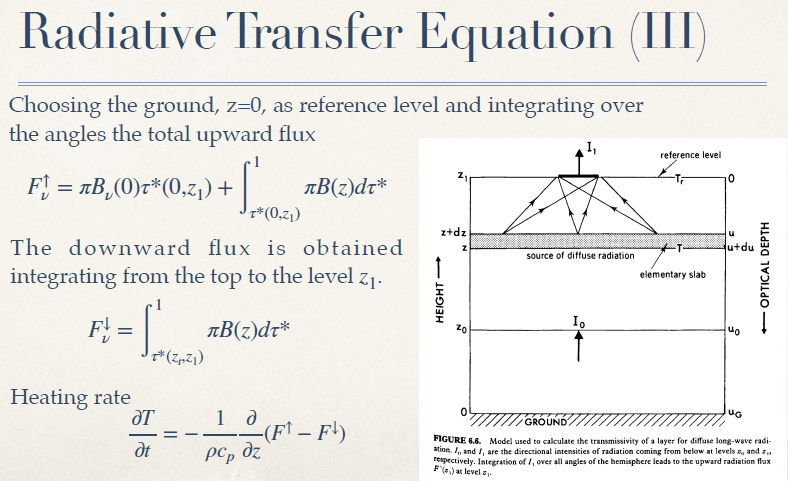
\includegraphics[width=0.5\linewidth]{uploads/18image.png}
	\caption{Enter Caption}
	\label{fig:enter-label}
\end{figure}

\paragraph{Solar radiation} The solar radiation is a function of the zenith angle
$$\cos Z = \sin \varphi \sin \delta + \cos \varphi \cos \delta \cos H$$

where $\varphi$ is latitude, $\delta$ is solar declination, which is the angular distance of the sun north of the equator and varies from about 23.5° on June 22 to -23.5° on December 22 and H is the hour angle, which is the longitudinal distance from the point in question to the meridian of solar noon and therefore is 0 at any point experiencing solar noon.
The solar flux, $S$, entering at the top of the atmosphere is a function of $\cos Z$ and the distance from the sun to the Earth, $d$, such that
$$S = S_0 f(d) \cos Z$$
where $S_{0}$ is the so-called solar constant (the solar energy flux received at the outer atmosphere on a surface normal to the solar beam; known now not to be constant) and the factor $f(d)$ is $1.0344$ in early January and $0.9674$ in July for the present astronomical conditions.
\begin{figure}[htp!]
	\centering
	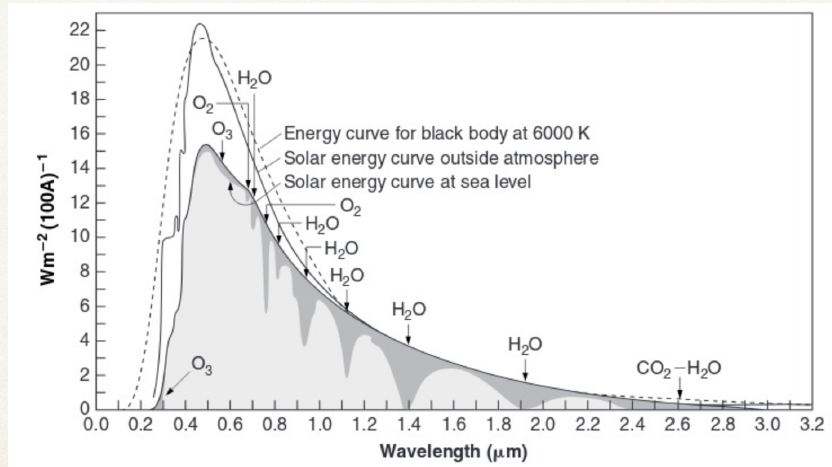
\includegraphics[width=0.5\linewidth]{uploads/image12.png}
	\caption{Spectral energy distribution as a function of wavelength at the top of the atmosphere and at sea level. The figure includes absorption by various atmospheric gases}
	\label{fig1}

\end{figure}
As shown in \ref{fig1} the principal absorber in the atmosphere is the stratospheric ozone, which absorbs very effectively in the ultraviolet and in the visible. Water vapor is the primary absorber in the troposphere in the near-infrared, also with carbon dioxide are the main important absorbers for the longer wavelengths.

\begin{figure}[htp!]
	\centering
	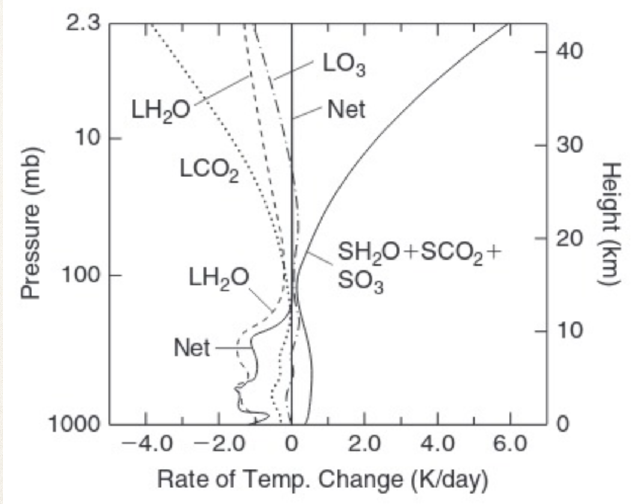
\includegraphics[width=0.4\linewidth]{uploads/image13.png}
	\caption{Heating rates in the atmosphere due to the absorption of solar radiation by atmospheric gases and due to the longwave or infrared radiation}
	\label{figl}
\end{figure}
The largest contributors to the eating/cooling rates are water vapor, carbon dioxide and ozone as shown in Figure \ref{figl}.
The net heating/cooling is zero in the stratosphere because in the one-dimensional model, it is in radiative equilibrium. The troposphere shows a net radiative cooling that is compensated by the vertical transfer of sensible and latent heat from below by moist adiabatic convection. As suggested in Figure \ref{figl} water vapor is the strongest contributor to the troposphere cooling. In the stratosphere cooling due to water vapor, carbon dioxide and ozone is generally compensated by heating due to absorption of solar radiation by zone.

\subsection{Moisture}
In order to discuss precipitation and cloud physics used in climate models, let's introduce basic concepts.
\textit{Moisture} is the quantity of water vapor in the air and it can be specified in several ways, depending on which reference is used.
\begin{itemize}
	\item \textit{mixing ratio} ratio of the density of water vapor to the density of dry air $q=\frac{\rho_w}{\rho}$
	\item \textit{specific humidity} ratio concerning the density of moist air, the density of water vapor over the total density of the air: $h=\frac{\rho_w}{q_w+\rho}$
	\item \textit{relative humidity} ratio of the mixing ratio to the saturation mixing ratio $r=\frac{q}{q_s}$
\end{itemize}
The same as the continuity mass treatment, the changes in the amount of water vapor must be balanced by the moisture sources and sinks
\begin{equation}\label{eqmpis}
	\frac{dq}{dt}= \frac{1}{\rho}M + E
\end{equation}

where M is the time rate change of water vapor per unit volume due to condensation or freezing (sinks of moisture) and E is the time rate of change of water vapor content per unit mass due to evaporation from the surface and sub-grid vertical and horizontal diffusion of moisture within the atmosphere (source of moisture). The first term on the right is a sink of moisture, the second is a source of moisture.
Often \ref{eqmpis} is written in flux form by combining with the continuity equation to obtain

\begin{equation}\label{eq4}
	\frac{\partial (\rho q)}{\partial t} + \nabla \cdot (\rho q \vec{V}) + \frac{\partial (\rho q \omega)}{\partial z} = M + \rho E
\end{equation}

If \ref{eq4} is integrated over the entire volume of the atmosphere, the second and the third terms on the left drop out, so that the sources and sinks of moisture must balance to have no secular change in atmospheric moisture over the globe.
If the atmosphere is saturated with moisture, then sensible heat can be added to the atmospheric system from latent heat by the conversion of water vapor to liquid warmer or ice parcels.

The first law of thermodynamic must incorporate in the nonadiabatic term, this energy conversion process due to phase changes between liquid, solid, and gas.
If the nonadiabatic process of conversion of water vapor to liquid water is the only energy source incorporated, the first law of thermodynamics becomes
$$c_p \, dT + \frac{1}{\rho} \, dp = - L \, dqs$$
The equation of state can be written like $$e = \rho_{W} RT$$ where $e$ is the partial pressure for water vapor.
Substituting in the previous equation, the mixing ratio becomes now
\begin{equation}\label{eq2}
	q\approx 0.622 \frac{e}{p}
\end{equation}

Inserting a total differential form of the hydrostatic equation, the first law of thermodynamics becomes $$\frac{dT}{dz} = - \frac{g}{c_p} - \frac{L}{c_p} \frac{dqs}{dz}$$
taking the log and differentiating the previous equation \ref{eq2} we will obtain
$$\log q_s \approx \log 0.622 + \log e_s - \log p$$
$$\frac{1}{e_s} \frac{d e_s}{d z} = \frac{1}{q_s} \frac{d q_s}{d z} + \frac{1}{p} \frac{d p}{d z}$$
$$\frac{1}{e_s} \frac{d e_s}{d T} = \frac{1}{q_s} \frac{d q_s}{d z} - \frac{1}{p} g \rho$$

The Clausius-Clapeyron equation relates the change in saturation vapor pressure to the latent heat involved in a phase change from water vapor to liquid water or from liquid water to ice. The most convenient form of this is $$\frac{1}{e_s} \frac{d e_s}{d T} = \frac{L}{R T^2}$$
So we get $$\frac{d q_s}{d z} = \frac{L q_s}{R W T_2} \frac{d T}{d z} + \frac{g q_s}{R T}$$

\begin{equation}\label{eq.adiabatic lapse rate}
	\Gamma_m= \frac{dT}{dz} = -\frac{g}{c_p} \left( 1 + \frac{L q_s}{R T} \right) \left( 1 + \frac{L^2 q_s}{c_p R W T_2} \right)^{-1}
\end{equation}
In this way, we will obtain the moist adiabatic lapse rate $\Gamma_m$, which is less than the adiabatic lapse rate defined earlier: $$\Gamma=\frac{dT}{dz}=-\frac{k\rho g}{p}T$$



\subsection{Clouds}
They play a critical role in the radiation characteristics of the Earth's climate, but their radiative properties are not fully understood. In most climate models, the precipitation and convective aspects of the model are used to compute where clouds exist based on whether the atmosphere is near saturation and whether convection is occurring. You can use different parameters to explain that.

\subsubsection{Cumulus formation}
If a parcel of air near the Earth's surface (at an atmospheric pressure of approximately 1000 mb) starts to rise, say from strong heating, it will cool at approximately the dry adiabatic lapse rate of 9.8 Kkm-¹. When the parcel cools sufficiently the parcel is saturated, gaining a condition of instability because there is much more energy in the water vapor. The level at which this occurs is termed the lifting condensation level, LCL, and is typically at the cloud base as the picture below shows.
\begin{figure}[htpb]
	\centering
	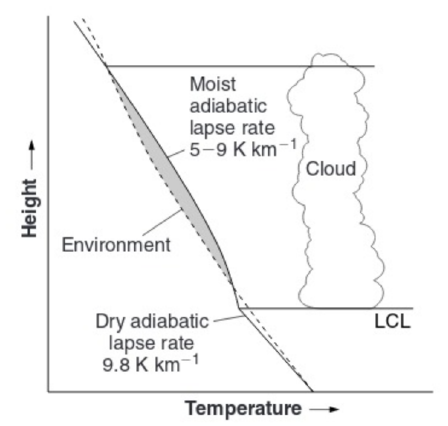
\includegraphics[width=0.4\linewidth]{uploads/image14.png}
	\caption{Enter Caption}
	\label{fig:enter-label}
\end{figure}
If the parcel does not rise high enough to reach an LCL, then a cloud should not form. From the LCL upward, the parcel will cool less rapidly as it rises since the latent heat of condensation or fusion releases heat. This lessened rate of temperature decrease with height is the moist adiabatic lapse rate.

\begin{figure}[htpb]
	\centering
	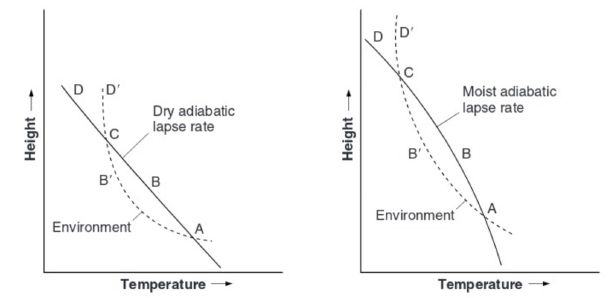
\includegraphics[width=0.5\linewidth]{uploads/image15.png}
	\caption{Diagram of stable and unstable conditions concerning dry and moist lapse rates.}
	\label{fig: figure 15}
\end{figure}
As shown in figure \ref{fig: figure 15} the dotted curve represents conditions for the environmental air, and the solid curves represent conditions for the path along which a parcel will ascend from point A to B, depending on whether the dry or the moist adiabatic lapse rate is appropriate. There is a point B' highlighted on the curve for the environmental air that is colder in both cases than point B for the parcel at the same height. Since the air at B' is colder than that at B, the parcel will have positive buoyancy. Thus in principle, it will continue ascending. If on the other hand, a parcel is at C and ascends to point D, it will be colder than the surrounding environmental air at D'. Thus the parcel will have negative buoyancy, which will cause it to sink to its original position.

\subsection{Surface Processes}
Boundary fluxes for momentum and heat, we can physically represent as
$$\tau_x = \rho C_D \left| \vec{v} - \vec{v_s} \right| (u_s - u)$$
$$\tau_y = \rho C_D \left| \vec{v} - \vec{v_s} \right| (v_s - v)$$
$$H = \rho c_p C_H \left| \vec{v} - \vec{v_s} \right| (\theta_s - \theta)$$
$$LE = \rho L_C E \left| \vec{v} - \vec{v_s} \right| (q_s - q)$$

Where over land $\vec{v}$ is zero.

Above the surface boundary layer adjacent to Earth's surface exists the planetary boundary layer, where the wind turns with the height. Within this region, the balance of forces can be approximated by Coriolis, pressure gradient, and frictional forces through the following simplification
$$-f_{\nu} = - \frac{1}{\rho a \cos \varphi} \frac{\partial p}{\partial \lambda} + F_{\lambda}$$
$$f_u = - \frac{1}{\rho a} \frac{\partial p}{\partial \varphi} + F_{\varphi}$$

The frictional term can be expressed as the vertical gradient of stress, so that $$F_\lambda = \frac{1}{\rho} \frac{\partial \tau_\lambda}{\partial z}$$
and $$F_\varphi = \frac{1}{\rho} \frac{\partial \tau_\varphi}{\partial z}$$


and the stress can in turn be related to the vertical gradient of wind shear
$$\tau_\lambda = \rho K_m \frac{\partial u}{\partial z}$$
and $$\tau_\varphi = \rho K_m \frac{\partial v}{\partial z}$$

where Km is the vertical eddy or transfer coefficient for momentum. Note that if the vertical wind shear is large, as one would expect near the Earth's surface since the wind must approach zero at the surface, then the momentum transfer is also large. On the molecular scale, Km, takes on values appropriate for those space scales; however, in the atmosphere and ocean models the space scales are much larger. Many of the eddies have dimensions of the order of the spatial grid structure of the models.
If the layer is unstable there is strong vertical mixing and Km is large; if the layer is stable there is no strong coupling and Km is small. A useful measure of this stability is the Richardson number $Ri$, which is defined as
$$R_i = \frac{g}{\theta} \frac{\frac{\partial \theta}{\partial z}}{\left( \frac{\partial V}{\partial z} \right)^2}$$
where $V = \left| \vec{V} \right|$ and $\frac{\partial V}{\partial z}$ is the vertical wind shear or vertical gradient of wind velocity.

\subsection{Hydrology}
\begin{figure}[htp!]
	\centering
	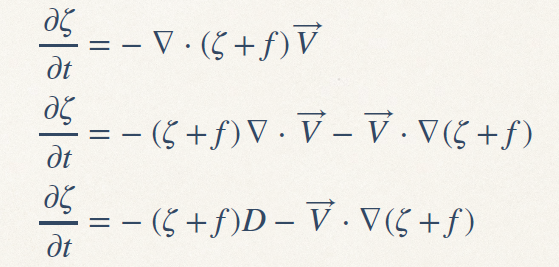
\includegraphics[width=0.5\linewidth]{uploads/15image.png}
	\caption{Schematic processes and features relevant to surface hydrology and evapotraspiration}
	\label{fig: fig 2}
\end{figure}
As shown in \ref{fig: fig 2} lots of processes are involved in surface hydrology. These include radiation, sensible heat, evaporation, transpiration, momentum, and precipitation, but also H2O and CO2 fluxes. The surface moisture can contribute to surface flow in streams percolate to a deeper layer or even become groundwater, depending on the porous properties of the ground. In the root zones of plants, some of the surface moisture can be taken up by the plant roots and then relayed to the plant leaves and transpired.

Within a land area as large as a horizontal grid cell of a global model, there are generally multiple surface types, including lakes, wetlands, different vegetation types, and different soil types
Another aspect of land surface processes being improved in many climate models is the simulation of snow coverage. The snow modeling community has developed a variety of models that can be used for climate and hydrology. These models range from the simple to the complex, and several of them are specifically designed for use in general circulation models. The more complex snow models take into account melting processes, grain size, shape, liquid water content, and percolation processes.


